\documentclass[12pt]{article}

\usepackage[brazil]{babel}   
\usepackage[utf8]{inputenc}  
%\usepackage[T1]{fontenc}
\usepackage{amsfonts,amsmath,amssymb,latexsym} 
\usepackage{graphicx}
\graphicspath{ {images/} }

\def\cQ{\mathcal{Q}}
\def\ve{\varepsilon}

\def\emptyset{\varnothing}


\title{Lista 01 de ATC}
\date{2º Período de 2023}
\author{Turma do 3º ano}

\begin{document} 


\maketitle

\begin{description}

\item[Definição de um Autômato Finito Não-Determinístico (AFN)]
\[A = (\cQ, \Sigma, \delta, q_0, F)\]
\begin{itemize}
\item Um conjunto de estados finito, $\cQ$
\item Um conjunto de símbolos de entrada $\Sigma$
\item Uma função de transição $\delta: \cQ\times\Sigma\rightarrow 2^\cQ$.
\item Um estado inicial $q_0$
\item Um conjunto de estados finais $F\subseteq \cQ$
\end{itemize}


\item[$2^\cQ$] é o conjunto de subconjuntos do conjunto $\cQ$


\end{description}


\vspace{3em}


\break



\begin{enumerate}

\item Forneça autômatos finitos não-determinísticos que aceitam as seguintes linguagens no alfabeto $\{0,1\}$. Você pode desenhar um diagrama de transições (o grafo) ou desenhar a tabela de transições. Dica: não precisa nomear os estados.

\begin{enumerate}

\item string que termina em 00

\item string que tem três 0's consecutivos

\item string que tem 011 como substring

\item tem 0101 como substring

\item tem 01 e 10 como substring

\item antes de cada 0 tem um 1.

\item strings que terminam em 01:

%\item não tem 00 como substring

%\item não tem 00 nem 11 como substring

\item é construído concatenando 01's e 010's e nenhum outra string

\end{enumerate}

\item Forneça autômatos finitos não-determinísticos que aceitam as seguintes linguagens. Você pode desenhar um diagrama de transições (o grafo) ou desenhar a tabela de transições.
\begin{enumerate}

\item No alfabeto $\{1,2,3\}$, strings tal que o dígito final tenha aparecido antes.

\item No alfabeto $\{1,2,3\}$, strings tal que o dígito final NÃO tenha aparecido antes.

\end{enumerate}





\break





\item Quais das seguintes strings são aceitos pelos autômatos determinísticos relacionados.

\begin{enumerate}

\item O autômato da figura \ref{fig:auto01}:

\begin{figure}[h]
    \centering
    \includegraphics[width=0.25\textwidth]{l02fig01}
    \caption{Autômato 01}
    \label{fig:auto01}
\end{figure}

\begin{enumerate}
\item $a$
\item $aa$
\item $aab$
\item $\varepsilon$
\end{enumerate}

\item O autômato da figura \ref{fig:auto02}:

\begin{figure}[h]
    \centering
    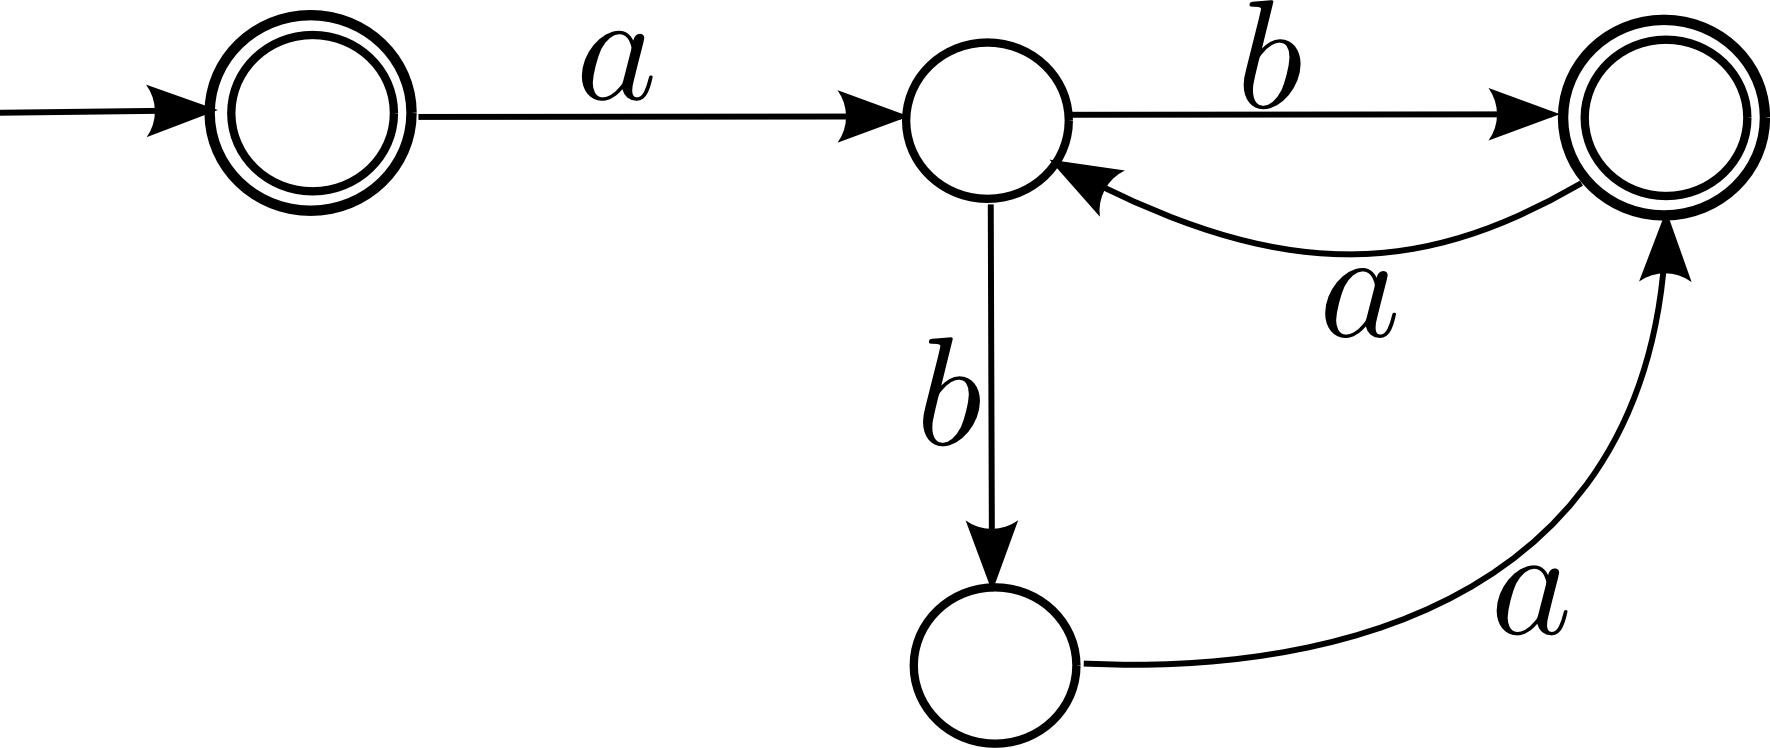
\includegraphics[width=0.40\textwidth]{l02fig02}
    \caption{Autômato 02}
    \label{fig:auto02}
\end{figure}

\begin{enumerate}
\item $\varepsilon$
\item $ab$
\item $abab$
\item $aba$
\item $abaa$
\end{enumerate}



\end{enumerate}



\end{enumerate}

\end{document}

